
\documentclass{article}


\usepackage[utf8]{inputenc} % allow utf-8 input
\usepackage[    % For using .bib file
backend=biber,
style=alphabetic,
sorting=ynt
]{biblatex}

\addbibresource{references.bib}


% if you need to pass options to natbib, use, e.g.:
%     \PassOptionsToPackage{numbers, compress}{natbib}
% before loading neurips_2023


% ready for submission
\usepackage[final]{neurips_2023}


% to compile a preprint version, e.g., for submission to arXiv, add add the
% [preprint] option:
%     \usepackage[preprint]{neurips_2023}


% to compile a camera-ready version, add the [final] option, e.g.:
    % \usepackage[final]{neurips_2023}


% to avoid loading the natbib package, add option nonatbib:
   % \usepackage[nonatbib]{neurips_2023}


\usepackage[T1]{fontenc}    % use 8-bit T1 fonts
\usepackage{hyperref}       % hyperlinks
\usepackage{url}            % simple URL typesetting
\usepackage{booktabs}       % professional-quality tables
\usepackage{amsfonts}       % blackboard math symbols
\usepackage{nicefrac}       % compact symbols for 1/2, etc.
\usepackage{microtype}      % microtypography
\usepackage{xcolor}         % colors
\usepackage{graphicx}


\title{Comparing Perceptual Quality vs. Pixel Loss on a Simple Video Super-Resolution Model}

% The \author macro works with any number of authors. There are two commands
% used to separate the names and addresses of multiple authors: \And and \AND.
%
% Using \And between authors leaves it to LaTeX to determine where to break the
% lines. Using \AND forces a line break at that point. So, if LaTeX puts 3 of 4
% authors names on the first line, and the last on the second line, try using
% \AND instead of \And before the third author name.


\author{
  Chad Weatherly \\
  Department of Computer Science \\
  University of Houston \\
  Houston, TX, USA \\
  \texttt{cdweathe@central.uh.edu} \\
  % examples of more authors
  \And
  Paramjit S. Kainth \\
  Department of Mechanical Engineering \\
  University of Houston \\
  Houston, TX, USA \\
  \texttt{pskainth@central.uh.edu} \\
  \And
  Abhigna Sowgandhika Vadlamudi \\
  Department of Computer Science \\
  University of Houston \\
  Houston, TX, USA \\
  \texttt{avadlam2@central.uh.edu} \\
  % \And
  % Coauthor \\
  % Affiliation \\
  % Address \\
  % \texttt{email} \\
  % \And
  % Coauthor \\
  % Affiliation \\
  % Address \\
  % \texttt{email} \\
}

\begin{document}

\maketitle

\begin{abstract}
 Needs to be completed last
\end{abstract}

\section{Introduction}

 Within the last decade, deep learning (DL) has been used in an attempt to solve the problem of Single Image Super-Resolution (SISR), which takes a low resolution (LR) image and attempts to construct a corresponding high resolution (HR) image. This problem was introduced to the mainstream with NVIDIA’s introduction of Deep Learning Super-Sampling (DLSS) in their GPU’s for playing video games. DLSS is more of a Video Super-Resolution (VSR) task, which gives more complexity to the SISR issue by introducing inter-frame information. The VSR task can be described as the reconstruction of high-resolution (HR) videos when only given low-resolution (LR) counterpart video. In the video game landscape, there is currently a drive to have games played at a high frame rate and with high resolution and video fidelity. This is extremely computationally expensive due to the sheer number of physics calculations each second. Improvements have been added every year or so since its inception in 2019. AMD and Intel have since introduced their own rival version of this type of model software, Fidelity SuperResolution (FSR) and XeSS, respectively, demonstrating the growth in this field in the past 3-4 years. The DLSS problem can also be transposed to other fields besides video games, such as “medical imagery reconstruction…remote sensing…panorama video super-resolution…surveillance systems…high-definition television” \cite{liu_video_2022}. 

\subsection{Prior Work}
 
Up until this point, there have been a few notable papers that have introduced new architectures to the field, based on other DL structures \cite{chan_basicvsr_2021}, \cite{chan_basicvsr_2022}, \cite{liang_recurrent_nodate}, \cite{rota_enhancing_2023}, with most all papers using similar datasets like Vimeo-90K \cite{xue_video_2019} and REDS \cite{nah_ntire_2021}. Notably, significant improvements have been found by introducing deformable convolutions \cite{dai_deformable_2016}, but most improvements come by training models to reduce pixel-loss functions, which often does not result in images that appear better to the human eye. Perceptual Quality (PQ) was introduced as a metric for image/video restoration problems \cite{johnson_perceptual_2016}, \cite{zhang_unreasonable_2018}, which aims for a chosen model architecture to have similar feature maps to those of other state-of-the-art (SOTA) image/CNN models, thereby enhancing perceptual quality. To explain this concretely, imagine a new DL model that needs to be trained for a VSR task. Given a LR frame/image, it will try to create a corresponding HR frame.  This is done by passing both the ground truth and predicted HR frame through a given model that performs well on image-related tasks (VGG, ImageNet, ResNet, ...). The loss measures the difference between the activation maps (tensors) created by passing both frames through this model. The idea is that if two images are perceptually similar, they will "look" similar to a model that performs well on extracting features from images, i.e. the goal is for the hidden features of two images to be similar, instead of just a pixel-to-pixel recreation. In testing, perceptual loss tends to create images that look "better" to human observers \cite{zhang_unreasonable_2018}. \\ % These two lines are used for adding space after a paragraph

Frustratingly, the training process is little emphasized in current SOTA VSR models, which is bizarre, as pixel-loss functions (like MSE) don’t capture the problem in its entirety, making the problem ill-posed. Many of the most cited papers for VSR tasks emphasize updated architectures, rather than viewing the VSR task holistically \cite{liu_video_2022}. In most cases, a model's acceptability is judged based on two criteria: Peak Signal-Noise Ratio (PSNR) and Structural Similarity Matrix (SSIM), as defined below for any two given images of the same size, \(\widetilde{I}\) and \(\hat{I}\): 

\begin{equation}
    SSIM(\widetilde{I}, \hat{I}) = \frac{
        2 \mu_{\hat{I}} \mu_{\widtilde{I}} + k_1}{
        \mu^2_{\hat{I}} + \mu^2_{\widetilde{I}} + k_1}
        \cdot
        \frac{
        2 \sigma_{\hat{I} \widtilde{I}} + k_2
        }{ \sigma^2_{\hat{I}} + \sigma^2_{\widetilde{I}} + k_2}
\end{equation}

where \(\mu_{\widetilde{I}} / \mu_{\hat{I}}\) and \(\sigma_{\widetilde{I}} / \sigma_{\hat{I}}\) are the mean and standard deviation, respectively, of image \(\widetilde{I}\) / \(\hat{I}\), \(\sigma_{\hat{I} \widetilde{I}}\) is the covariance of the two images, and \(k_1\) and \(k_2\) are constants, usually set to 0.01 and 0.03, respectively.

\begin{equation}
    PSNR(\widetilde{I}, \hat{I}) = 10*log_{10} \left( \frac{L^2}{MSE ( \widetilde{I}, \hat{I} )} \right)
\end{equation} 

where L represents the maximum range of color values, which is usually 255, and the Mean-Squared Error (MSE) is defined as: 

\begin{equation}
    MSE(\widetilde{I}, \hat{I}) = \frac{1}{N} \sum^{N}_{i=1} (\widetilde{I}_i - \hat{I}_i)^2
\end{equation} 

for each pixel value \(i\) in all pixel values \(N\). 

\section{Problem Statement}

In this project, the aim is to assess how adjusting the training process to use perceptual loss might affect the final performance of a simple DL model trained on the VSR task. This projects strives to train a novel, but simple, VSR model, first on pixel-loss metrics, second using perceptual quality.  

\section{Technical Approach / Methodology}

Originally, the intention was to create a diffusion model, similar to the one by Rota et al. \cite{rota_enhancing_2023}, that would perform VSR on the REDS dataset \cite{nah_ntire_2021}, but this was changed for two reasons: the data necessitated a large model that was infeasible to train on a local machine, and the diffusion model needed much compute in order to be trained effectively. We did not have the time to feasibly train the model on this data. For these reasons, we decided to go with a simpler model architecture and a simpler data set, where individual frames were smaller.

\subsection{Data}

We chose to use the \href{https://www.cs.toronto.edu/~nitish/unsupervised_video/}{Moving MNIST} dataset, because its small frame size (64 x 64) was well suited to our task. Also, the fact that it only has one channel further motivated the decision. Each sample consists of 20 frames in a sequence, with 10,000 samples/videos in total. We used 8,000 samples for training and 2,000 for testing. \\

During training, for a given sample \(i\), a random sequence of 5 consecutive frames was chosen from the sample. These frames were downsampled using bicubic interpolation to be of size (32 x 32) and then processed through a Gaussian blur. These 5 images were passed to the model, with the aim of predicting the middle frame's HR counterpart. For a video sequence consisting of 20 frames, inference can be done by upsampling the central 16 frames.

\subsection{Model Architecture}

Due to the technical and time constraints of a class project, we propose to create our own network that would be effective in evaluating the loss/objective metrics, but simple enough to be trained on local machines. The model takes in 5 frames (as it will be a video), and the middle frame of these 5 is the one we wish to reconstruct as a HR image (Fig. 1). First, to capture feature information about each of the images, the 5 frames are each passed through 3 convolutional layers, where each layer is Max Pooled and activated using the Exponential Linear Unit (ELU, Eq. 4). Each image tensor is flattened to a 1-Dimensional vector. Then, the vectors are each reshaped to be size (32, 256). These 2D vectors are stacked as "channels", creating one image, which is finally passed through two more convolutional layers and activated with ReLU. Finally, the entire vector is flattened to 1D, and passed through a linear layer, which reduces its size to 4096. This final vector is reshaped to be size (64, 64) and passed as the output of the model. 

\begin{figure}
    \centering
    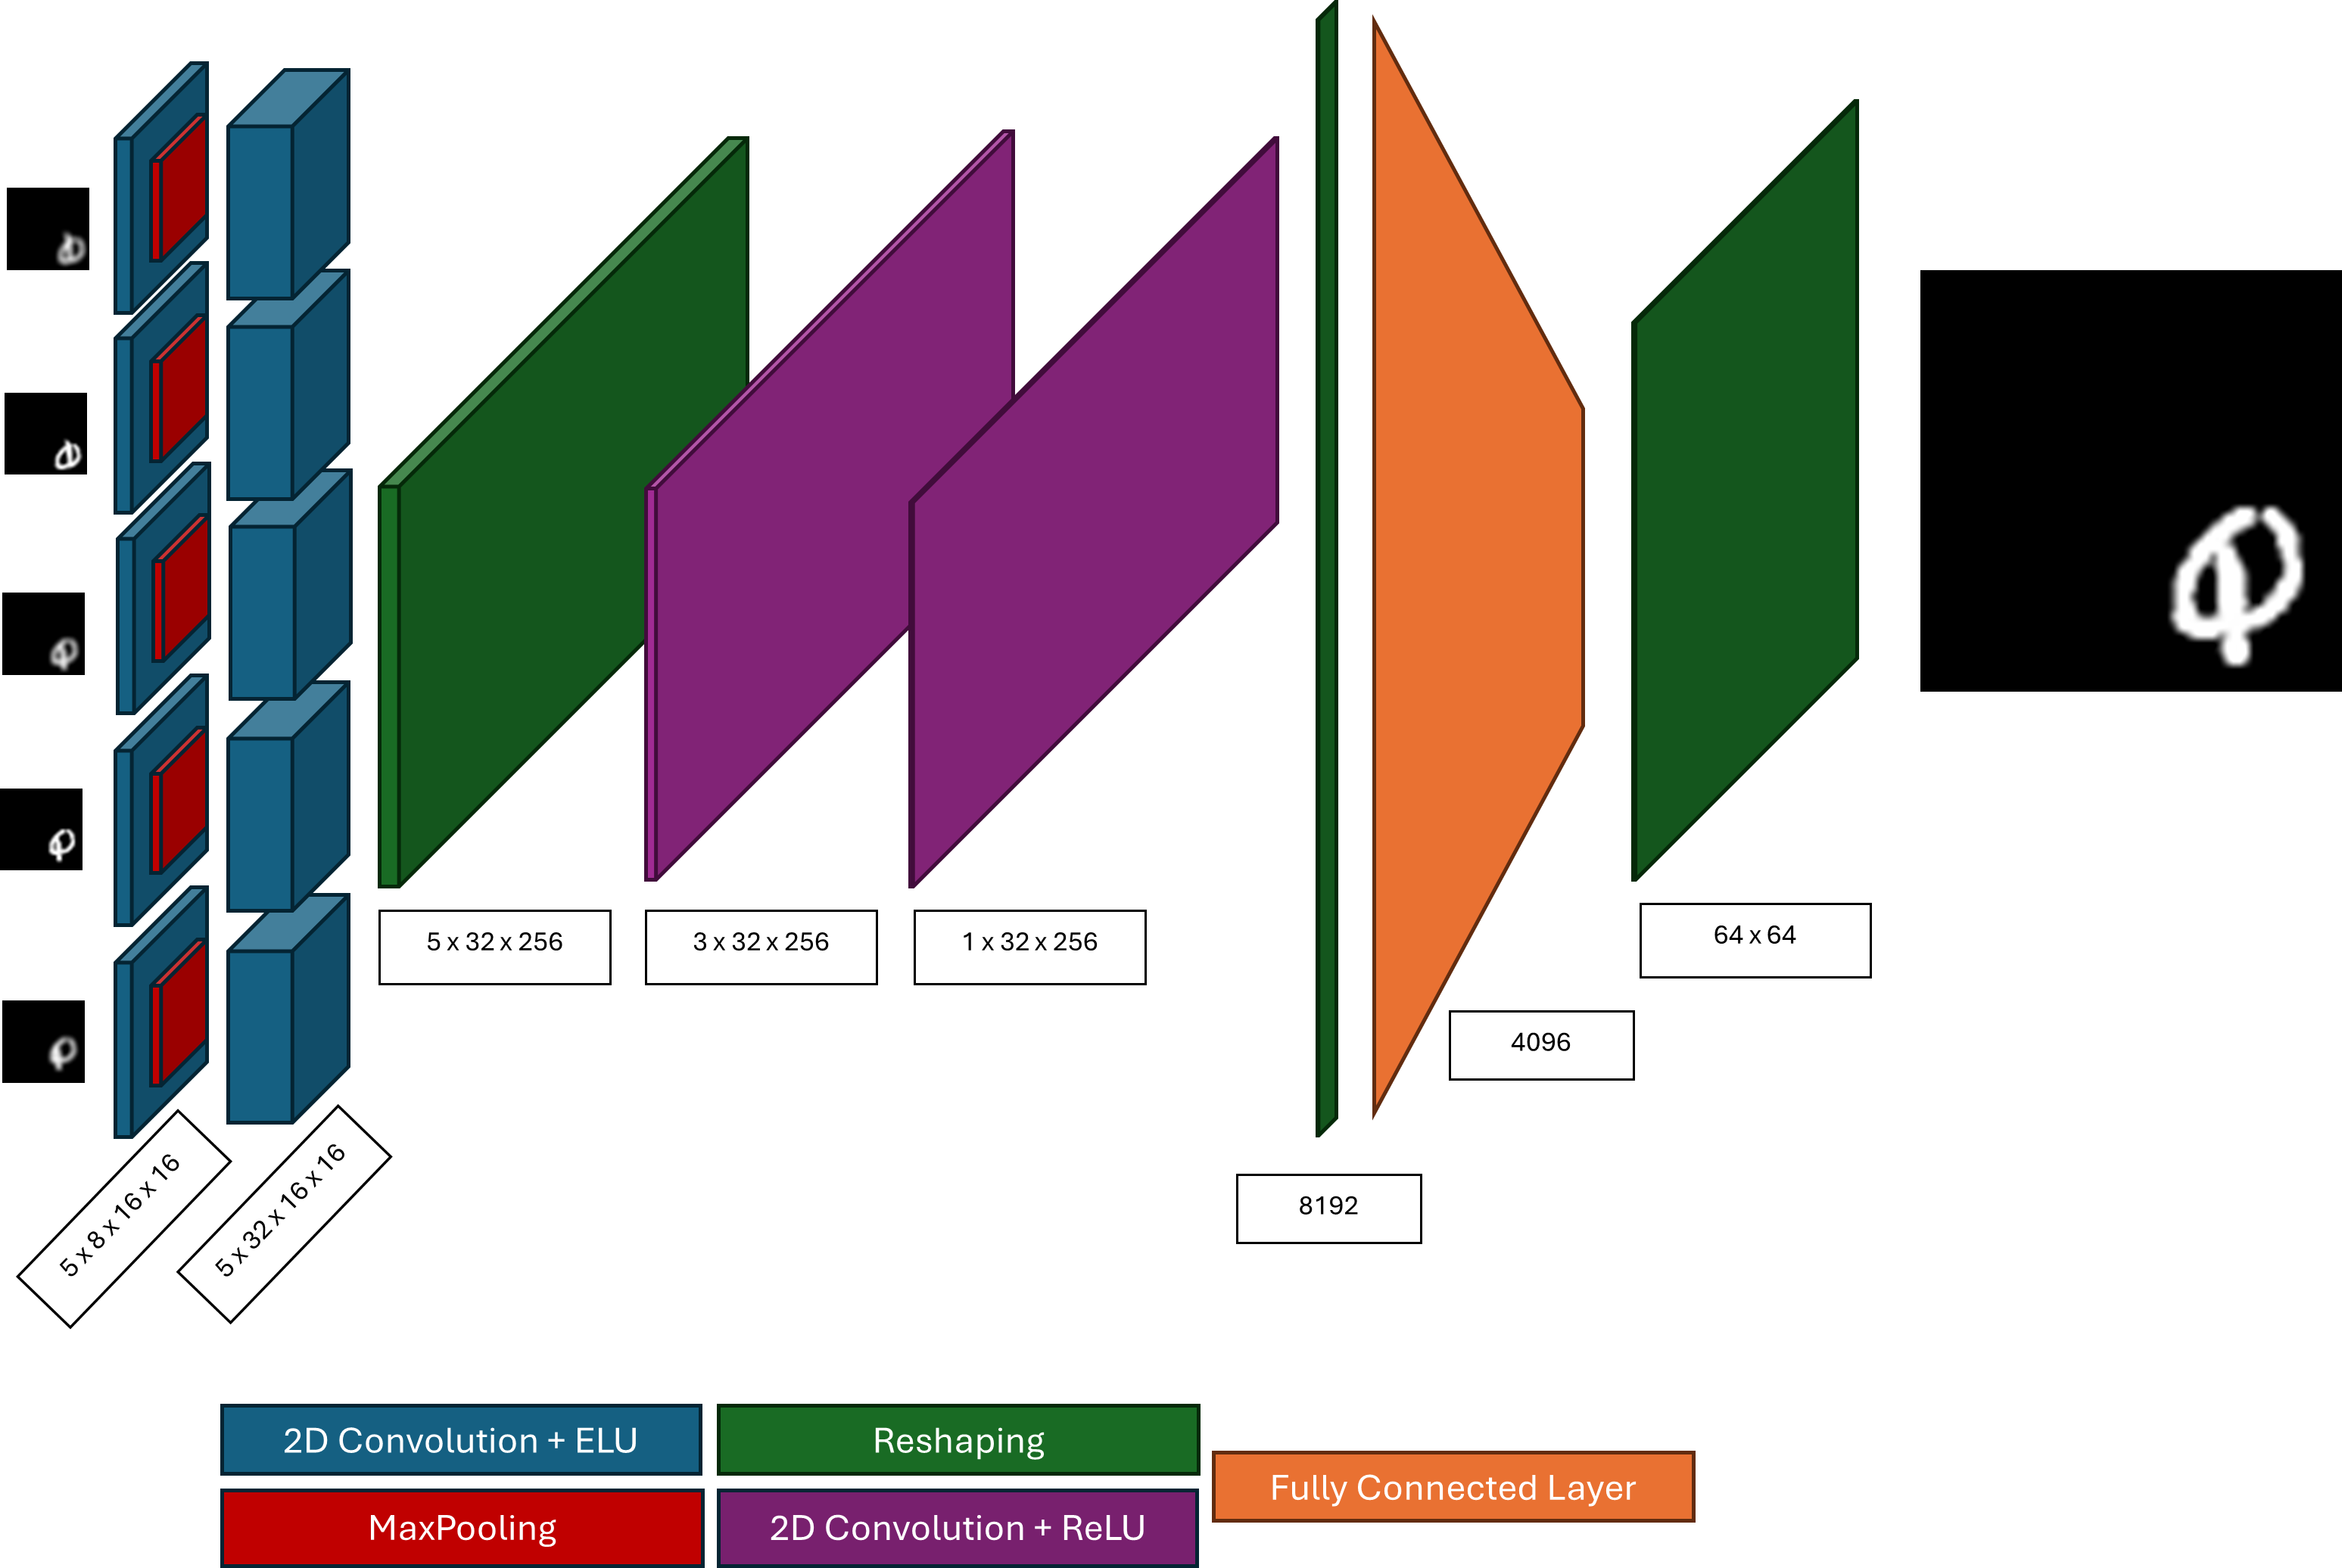
\includegraphics[width=1.0\linewidth]{model_architecture.png}
    \caption{Model Architecture}
\end{figure}

\begin{equation}
    ELU(x) = \left\{\begin{array}{lr}
       x,       & if \hspace{5} x > 0 \\
       e^x - 1, & if \hspace{5} x \leq 0
    \end{array}\right.
\end{equation}

\subsection{Training}

The novelty of our approach is found in the training process. We trained two versions of the model architecture (Fig. 1). Model 1 was trained on a perceptual loss metric (Eq. 5), as proposed by Johnson et al. \cite{johnson_perceptual_2016}. Our implementation of perceptual loss was done with the VGG-19 model \cite{simonyan_very_2015}, where activations were computed by passing each image (the ground truth and predicted HR images) and extracting the values from each ReLU activation. Model 2 was trained on the MSE (Eq.3) difference between the two image pixel values. Both models were trained on 50 epochs using the Adam optimizer. The learning rate was adjusted as epochs were passed: 0.0001 at start, 0.00001 after 5 epochs, and 0.000001 after 15 epochs.

\begin{equation}
    Perceptual \hspace{3} Loss(\hat{I}, \widetilde{I}) = \sum_{a=1}^N \Biggl[ \frac{1}{T} \sum_{t=1}^T \big| VGG_{a,t}(\hat{I}) - VGG_{a,t}(\widetilde{I}) \big| \Biggr]
\end{equation}

for \(T\) values in activation layers \(A\), where \(VGG_{a,t}(I)\) is the ReLU output value \(t\) from activation layer \(a\) when image \(I\) is passed through. 

\section{Results}

Figures 2 and 3 show how the loss functions converged for each of the 

\begin{figure}
    \centering
    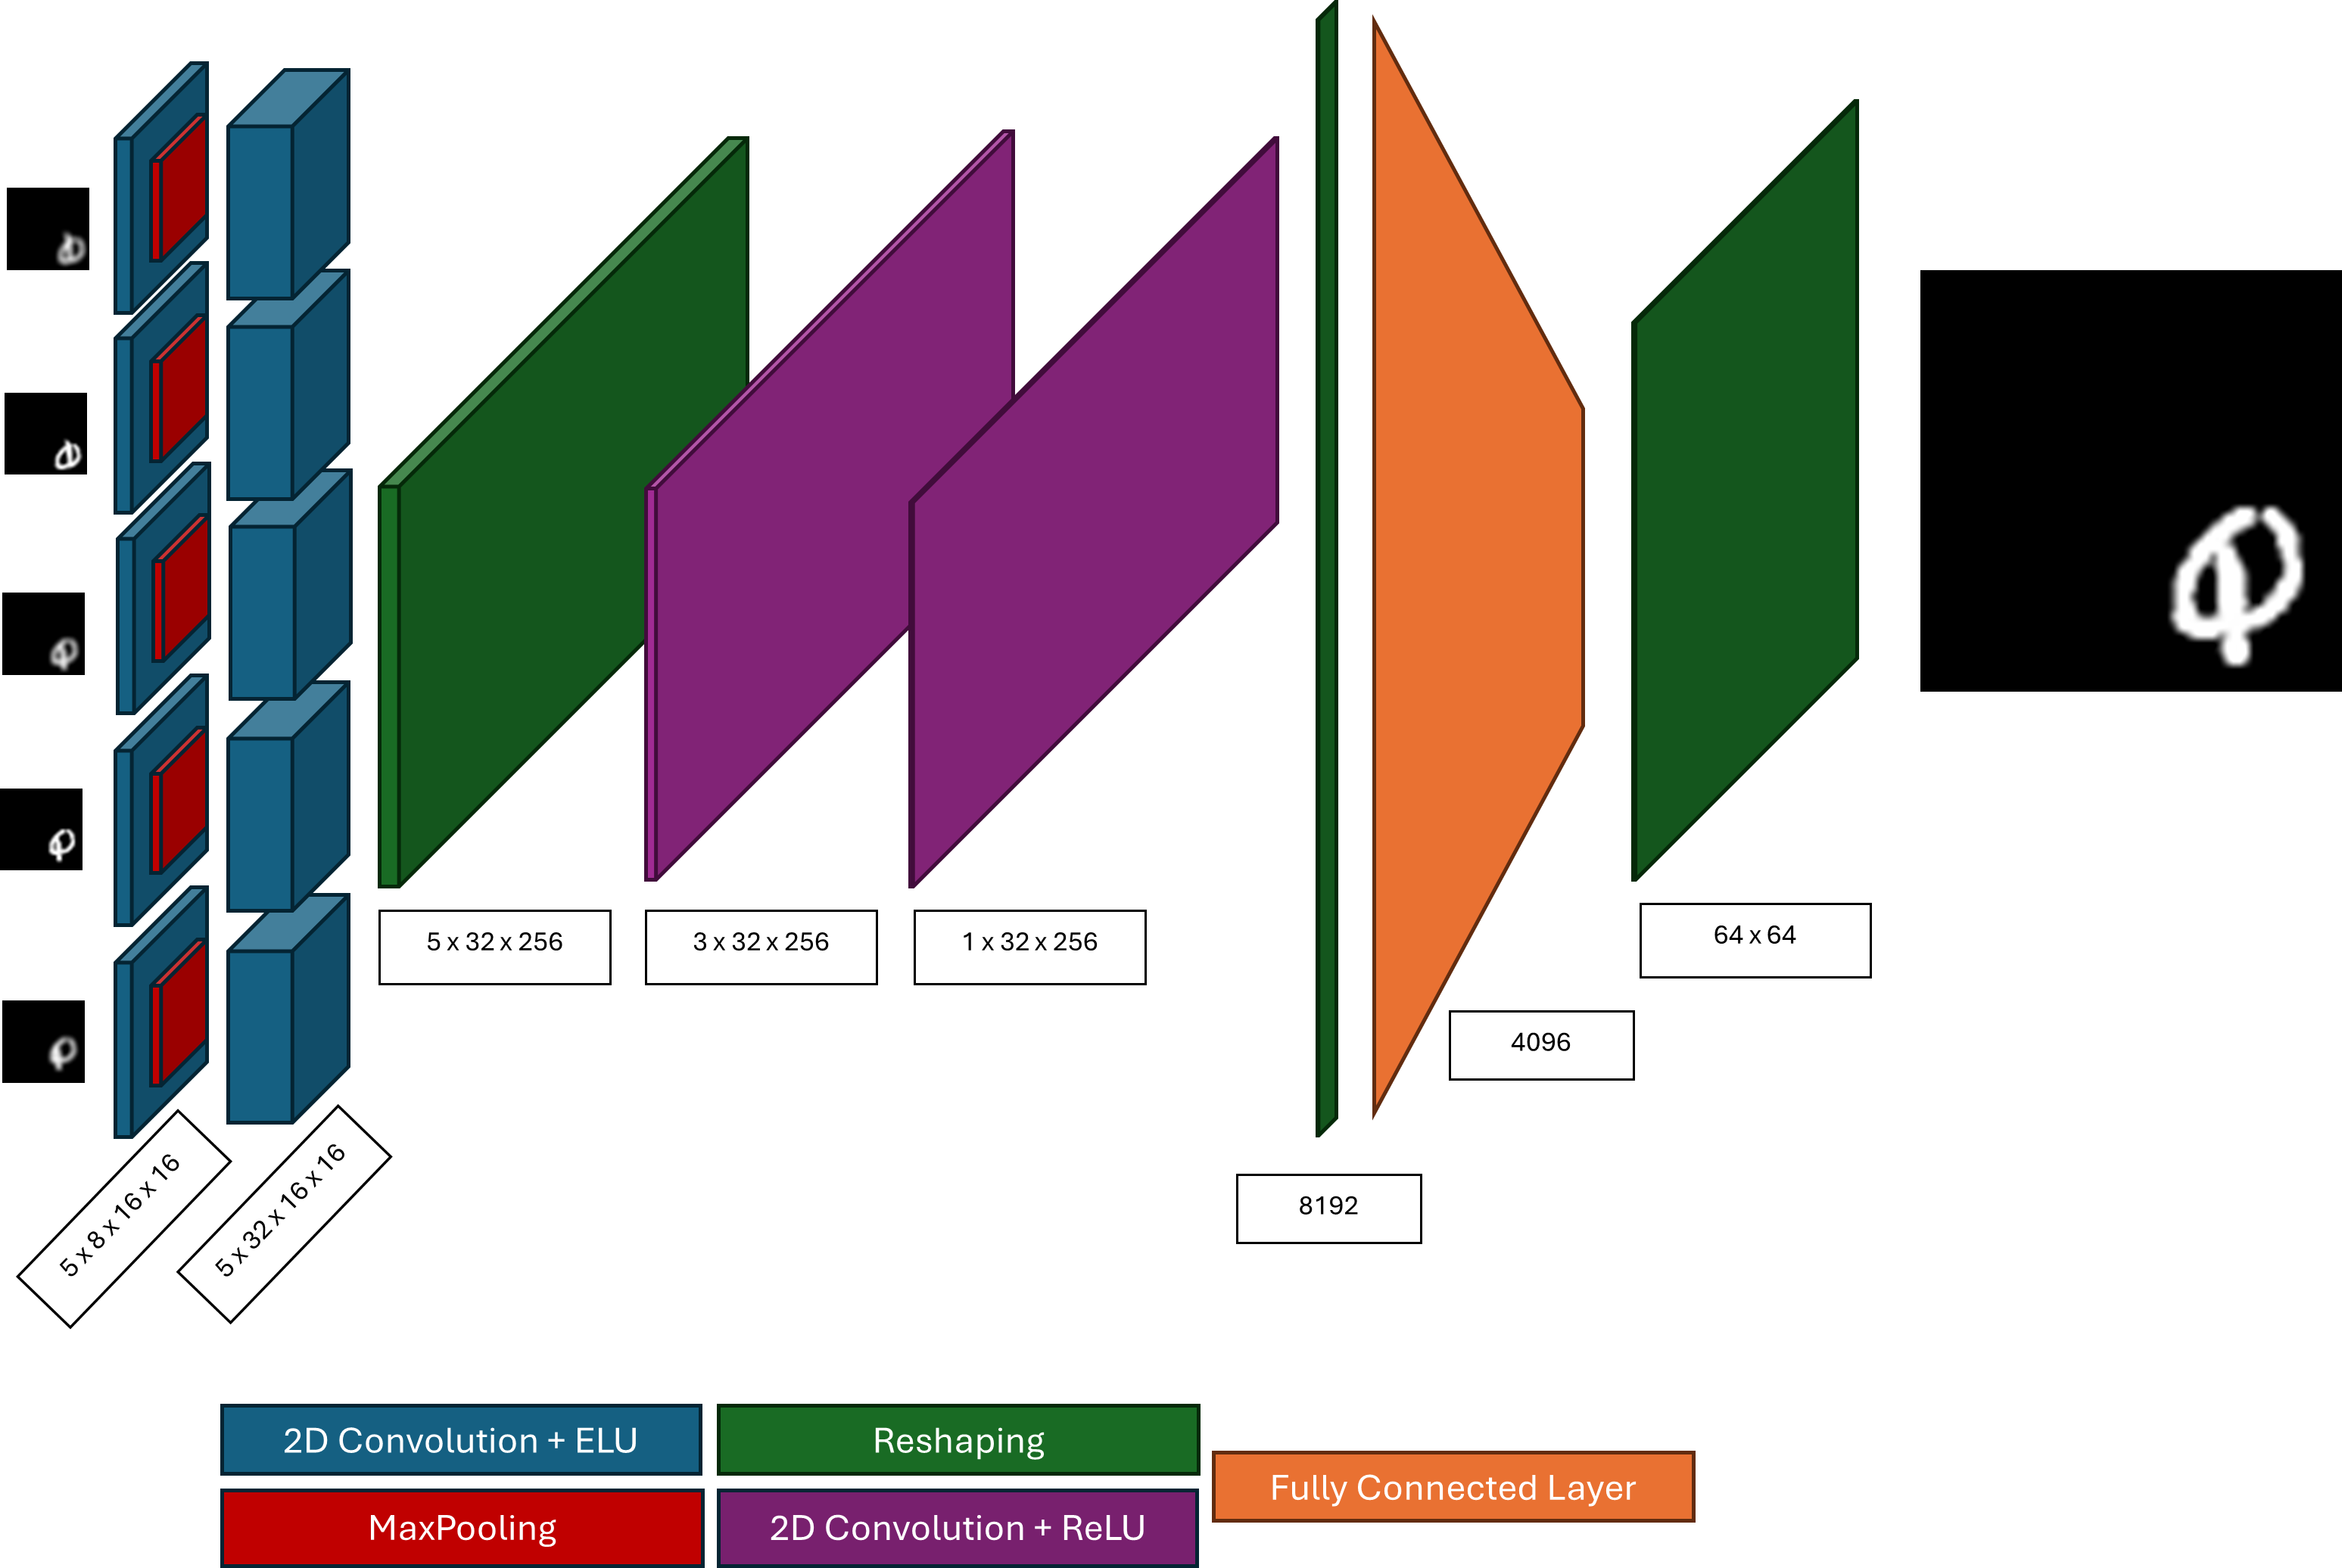
\includegraphics[width=1.0\linewidth]{model_architecture.png}
    \caption{Model Architecture}
\end{figure}

\section{Discussion}

\printbibliography % Prints all references cited using \cite{} in alphabetical order
%%%%%%%%%%%%%%%%%%%%%%%%%%%%%%%%%%%%%%%%%%%%%%%%%%%%%%%%%%%%


\end{document}